\documentclass[a4paper, 10pt, final, garamond]{book}
\usepackage{cours-preambule}

\makeatletter
\renewcommand{\@chapapp}{Chimie -- chapitre}
\makeatother

\hfuzz=5.002pt

% \toggletrue{student}
% \toggletrue{corrige}
% \renewcommand{\mycol}{black}
\renewcommand{\mycol}{gray}

\begin{document}
\setcounter{chapter}{5}

\settype{enon}
\settype{solu_prof}
\settype{solu_stud}

\chapter{\cswitch{Correction du TD}{TD~: oxydoréduction}}

\resetQ
\section{Équations bilan d'oxydoréduction}
\enonce{%
On s'intéresse aux couples
$\ce{{MnO_4^{-}}_{\rm(aq)}}/\ce{{Mn}^2+_{\rm(aq)}}$,
$\ce{HClO_{\rm(aq)}}/\ce{{Cl_2}_{\rm(aq)}}$ et
$\ce{{Cl_2}_{\rm(g)}}/\ce{Cl^-_{\rm(aq)}}$. On rappelle que $\ce{MnO_4^-}$ est
l'ion permanganate et \ce{HClO} l'acide hypochloreux.
}%

\QR{%
	Écrire et équilibrer les demi-équations de chacun des couples en milieu acide.
}{%
	\leavevmode\vspace*{-15pt}\relax
	\begin{alignat*}{4}
		\beforetext{On obtient}
		\ce{{MnO_4^{-}}_{\rm(aq)} & + 8 {H}^+_{\rm(aq)}      &  & +5e^- &  & = & {Mn}^2+_{\rm(aq)} & + 4 H_2O_{\rm(l)}}
		\\
		\ce{2{HClO}_{\rm(aq)}     & + 2 {H}^+_{\rm(aq)}      &  & +2e^- &  & = & {Cl_2}_{\rm(g)}   & + 2 H_2O_{\rm(l)}}
		\\
		\ce{                      & \wht{+2} {Cl_2}_{\rm(g)} &  & +2e^- &  & = & 2{Cl}^-_{\rm(g)}  & }
	\end{alignat*}
}%
\QR{%
	Lorsque la réaction est possible, écrire l'équation-bilan de la réaction
	entre~:
	\smallbreak
	\noindent
	\begin{minipage}[c]{.45\linewidth}
		\begin{enumerate}[label=\alph*)]
			\item L'acide hypochloreux et l'ion manganèse~;
			\item l'ion manganèse et l'ion chlorure~;
			\item l'ion manganèse et le dichlore~;
		\end{enumerate}
	\end{minipage}
	\hfill
	\begin{minipage}[c]{.45\linewidth}
		\begin{enumerate}[label=\alph*), start=4]
			\item le permanganate et le dichlore~;
			\item le permanganate et l'ion chlorure~;
			\item le dichlore sur lui-même.
		\end{enumerate}
	\end{minipage}
}{%
	\vspace{-15pt}
	\begin{enumerate}[label=\alph*)]
		\item Pas de difficulté~:
		      \[
			      \ce{10 HClO_{\rm(aq)} + 2 {Mn}^2+_{\rm(aq)} = 5 {Cl_2}_{\rm(g)} + 2
			      H_2O_{\rm(l)} + 2 {MnO_4^{-}}_{\rm(aq)} + 6 {H}^+_{\rm(aq)}}
		      \]
		\item Pas de réaction entre $\ce{Mn^2+}$ et $\ce{Cl^-}$ puisque ce sont deux
		      réducteurs.
		\item $\ce{Mn^2+}$ est un réducteur, donc $\ce{Cl_2}$ intervient en tant
		      qu'oxydant~:
		      \[
			      \ce{
			      2 {Mn}^2+_{\rm(aq)} + 8 H_2O_{\rm(l)} + 5{Cl_2}_{\rm(g)} =
			      2 {MnO_4^{-}}_{\rm(aq)} + 16 {H}^+_{\rm(aq)} + 10 {Cl}^-_{\rm(aq)}
			      }
		      \]
		\item Comme $\ce{MnO_4^{-}}$ est un oxydant, $\ce{Cl_2}$ intervient e tant
		      que réducteur~:
		      \[
			      \ce{2 {MnO_4^{-}}_{\rm(aq)} + 6 {H}^+_{\rm(aq)} + 5 {Cl_2}_{\rm(g)} =
			      2 {Mn}^2+_{\rm(aq)} + 10 HClO_{\rm(aq)}}
		      \]
		\item Pas de difficulté~:
		      \[
			      \ce{2 {MnO_4^{-}} + 16 {H}^+_{\rm(aq)} + 10 {Cl}^- _{\rm(aq)} =
			      2 {Mn}^2+_{\rm(aq)} + 8 H_2O_{\rm(l)} + 5 {Cl_2}_{\rm(g)}}
		      \]
		\item Le dichlore intervient en tant qu'oxydant et réducteur, c'est une
		      dismutation~:
		      \[
			      \ce{{Cl_2}_{\rm(g)} + H_2O_{\rm(l)} = {Cl}^-_{\rm(aq)} + HClO_{\rm(aq)}+
			      {H}^+_{\rm(aq)}}
		      \]
	\end{enumerate}
}%

\resetQ
\section{Nombres d'oxydation du chrome}
\enonce{%
	Le chrome \ce{Cr} a pour numéro atomique $Z = 24$, et il est moins
	électronégatif que l'oxygène.
}%
\QR{%
Donner le \no du chrome au sein des espèces $\ce{Cr_{\rm(s)}}$,
$\ce{{Cr}^2+_{\rm(aq)}}$ et $\ce{{Cr}^3+_{\rm(aq)}}$.
}{%
On fait attention à bien parler du nombre d'oxydation du chrome \textbf{dans
	l'édifice $\ce{Cr^2+}$}, et dans ce cas le \no est égal à la charge~:
\[
	\boxed{
		\no{Cr \in Cr} = 0
		\qquad
		\no{Cr \in Cr^2+} = +\myRoman{2}
		\qquad
		\no{Cr \in Cr^3+} = +\myRoman{3}
	}
\]
}%
\QR{%
	Sans représenter les schémas de \textsc{Lewis}, déterminer le \no du chrome
	dans les espèces \ce{CrO4^2-} et \ce{Cr2O7^2-}. On précise qu'il n'y a pas de
	liaison \ce{Cr-Cr} dans le dichromate.
}{%
	On suppose que $\no{O} = - \myRoman{2}$, puisque l'oxygène est l'élément le
	plus électronégatif et qu'il ne lui manque que 2 électrons pour remplir sa
	couche de valence. Avec la somme des \no qui doit être égale à la charge
	totale de l'édifice, on obtient
	\begin{itemize}
		\item $q (\ce{CrO_4^{2-}}) = -2 = \no{Cr} + 4 \no{O} \Lra \boxed{\no{Cr \in
			      CrO_4^{2+}} = + \myRoman{6}}$~;
		\item $q (\ce{Cr_2O_7^{2-}}) = -2 = 2 \no{Cr} + 7 \no{O} \Lra \boxed{\no{Cr
			      \in Cr_2O_7^{2-}} = + \myRoman{6}}$.
	\end{itemize}
}%
\QR{%
	Justifier que \ce{Cr2O7^2-} et \ce{Cr^3+} forment un couple rédox. Identifier
	l'oxydant et le réducteur sans utiliser la demi-équation. Écrire
	\textbf{ensuite} la demi-équation associée, en milieu acide et en milieu
	basique.
}{%
	Un couple rédox échange des électrons, donc les deux espèces \textbf{ont
		forcément des \no différents}~: c'est bien le cas du chrome dans le chrome III
	et du chrome dans les ions dichromates. On identifie l'oxydant comme étant
	celui de \no le plus élevé, ici \textbf{\ce{Cr2O7^{2-}} est l'oxydant}, et le
	réducteur comme celui de \no le plus bas, ici \textbf{\ce{Cr^3+} est le
		réducteur}. On obtient~:
	\begin{align*}
		\ce{
		2 {Cr}^3+_{\rm(aq)} + 7 H_2O_{\rm(l)}
		 & =
		{Cr_2O_7}^{2-}_{\rm(aq)} + 14 {H}^+_{\rm(aq)} + 6 e^-
		}
		\tag*{milieu acide}
		\\
		\beforetext{On ajoute \ce{14 HO-}}
		\ce{
		2 {Cr}^3+_{\rm(aq)} + 14 {HO}^-_{\rm(aq)}
		 & =
		{Cr_2O_7}^{2-}_{\rm(aq)} + 7 H_2O_{\rm(l)} + 6 e^-
		}
		\tag*{milieu basique}
	\end{align*}
}%
\QR{%
Justifier que \ce{CrO4^2-} et \ce{Cr2O7^2-} ne forment pas un couple rédox.
Montrer qu'il s'agit cependant d'un couple acide-base par écriture d'une
demi-équation.
}{%
Le chrome a le \textbf{même \no dans les deux cas}, donc ce n'est pas un
couple rédox. Par contre ils peuvent échanger des protons. Pour s'en assurer,
on équilibre la réaction comme d'habitude mais sans rajouter d'électrons~:
\[
	\boxed{\ce{
	{Cr_2O_7^{2-}}_{\rm(aq)} + H_2O_{\rm(l)} =
	2 {CrO_4^{2-}}_{\rm(aq)} + 2 {H}^+_{\rm(aq)}
	}}
\]
On a bien «~acide + eau = base + proton~», et pas d'électrons~: c'est un couple
acide-base~!
}%

% TODO: oubli du n.o. du soufre piqué à langevin

\resetQ
\section{Dismutation du dioxyde d'azote}
\enonce{%
En présence d'eau, le dioxyde d'azote $\ce{{NO_2}_{\rm(g)}}$ peut se dismuter
en ions nitrates $\ce{{NO_3}^-_{\rm(aq)}}$ et nitrites
$\ce{{NO_2}^-_{\rm(aq)}}$. Cette réaction produit des protons
$\ce{{H}^+_{\rm(aq)}}$, à l'origine des pluies acides.
}%
\QR{%
Écrire les demi-équations de transfert électronique et la relation de
\textsc{Nernst} pour les deux couples
$\ce{{NO_3^{-}}_{\rm(aq)}}/\ce{{NO_2}}_{\rm(g)}$ ($E_1^\circ = \SI{0.83}{V}$)
et $\ce{{NO_2}_{\rm(g)}/{NO_2^{-}}_{\rm(aq)}}$ ($E_2^\circ = \SI{0.85}{V}$).
}{%
On a~:
\begin{itemize}
	\item \leftcenters{%
	      $\ce{(NO_3^{-}_{\rm(aq)}/{NO_2}_{\rm(g)})}$~:
	      }{%
	      $\ce{{NO_2}_{\rm(g)} + H_2O_{\rm(l)} = {NO_3^{-}}_{\rm(aq)} +
		      2{H}^+_{\rm(aq)} + e^-}$
	      }%
	      \vspace{-15pt}
	      \[
		      \Ra
		      E_1 = E_1^\circ + \num{0.06} \log
		      \frac{[\ce{NO_3^{-}}][\ce{H^+}]^2p^\circ}{p_{\ce{NO_2}}{c^\circ}^3}
	      \]
	\item \leftcenters{%
	      $\ce{{NO_2}_{\rm(g)}/{NO_2^{-}}_{\rm(aq)}}$~:
	      }{%
	      $\ce{{NO_2^{-}}_{\rm(aq)} = {NO_2}_{\rm(g)} + e^-}$
	      }%
	      \vspace{-15pt}
	      \[
		      \Ra
		      E_2 = E_2^\circ + \num{0.06}\log \frac{p_{\ce{NO_2}}c^\circ}{p^\circ
		      [\ce{NO_2^{-}}]}
	      \]
\end{itemize}
}%
\QR{%
	Justifier à l'aide de diagrammes de prédominance que \ce{NO2} se dismute. On
	choisira $p_{\ce{NO_2}} = \SI{1}{bar}$ et une concentration frontière
	(convention de tracé) de $\SI{1}{mol.L^{-1}}$ à pH nul.
}{%
	\noindent
	\begin{minipage}[c]{.48\linewidth}
		On calcule les potentiels frontière connaissant la convention de tracé~:
		\begin{gather*}
			E\ind{1,front} = E_1^\circ + \num{0.06}\log c_t = E_1^\circ = \SI{0.83}{V}
			\\\beforetext{et}
			E\ind{2,front} = E_2^\circ + \num{0.06}\log c_t = E_2^\circ = \SI{0.85}{V}
		\end{gather*}
	\end{minipage}
	\hfill
	\begin{minipage}[c]{.48\linewidth}
		D'où le diagramme~:
		\begin{center}
			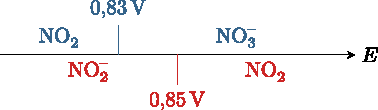
\includegraphics[width=.9\linewidth]{predom_no2}
		\end{center}
	\end{minipage}
	\smallbreak
	Ainsi, \textbf{les domaines de prédominance de \ce{NO2} sont disjoints}~: il
	va spontanément réagir avec lui-même pour donner des formes qui peuvent
	coexister au même potentiel, c'est-à-dire qu'il se dismute.
	\smallbreak
	On observe cependant que les potentiels frontières sont très proches, donc la
	réaction associée sera très limitée (grossièrement, il faut
	$\abs{\Delta{E\ind{lim}}} \approx \SI{0.20}{V}$ pour avoir totalité~; cela
	dépend du nombre d'électrons échangés mais sûrement avec une différence de
	$\SI{0.02}{V}$ on n'y est pas~!)
}%
\QR{%
Écrire l'équation bilan de l'équation de dismutation.
}{%
\centers{$\ce{2 {NO_2}_{\rm(g)} + H2O_{\rm(l)} = {NO_3^{-}}_{\rm(aq)} +
	{NO_2^{-}}_{\rm(aq)} + 2 {H}^+_{\rm(aq)}}$}
}%
\QR{%
	Exprimer sa constante d'équilibre $K^\circ$ en fonction des potentiels
	standard et calculer sa valeur numérique.
}{%
	On pourrait refaire le calcul du cours, mais ça n'est pas demandé~: on donne
	simplement
	\[
		K^\circ =
		10^{\DS +\frac{\abs{\Delta{E^\circ}}}{\num{0.06}}} =
		10^{\DS \frac{E_2^\circ - E_1^\circ}{\num{0.06}}}
		\Lra
		K^\circ = \num{2.15}
	\]
	en prenant la valeur absolue puisqu'on a déterminé que la réaction était
	favorisée à la question précédente (domaines disjoints $\Lra K^\circ > 1 \Lra$
	réaction favorisée). Elle est donc en effet favorisée, mais très peu, on a
	$K^\circ$ proche de l'unité, c'est cohérent.
}%

\resetQ
\section{Éthylotest}
\enonce{%
	\noindent
	\begin{minipage}[c]{.20\linewidth}
		\begin{center}
			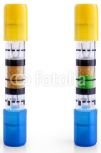
\includegraphics[width=\linewidth]{ethylotest}
		\end{center}
	\end{minipage}
	\hfill
	\begin{minipage}[c]{.75\linewidth}
		Peu après avoir été consommé, l'alcool (éthanol de formule \ce{CH3CH2OH})
		passe dans le sang au niveau de l'intestin grêle. Ensuite, des échanges
		gazeux s'effectuent dans les alvéoles pulmonaires~: le sang se charge en
		dioxygène et se libère du dioxyde de carbone, ainsi que d'une partie de
		l'alcool. Ces vapeurs sont expirées dans l'air avec une concentration en
		alcool \num{2100} fois inférieure à celle du sang. Le seuil limite autorisé
		pour la conduite est de \SI{0.50}{g} d'éthanol par litre de sang.
		\smallbreak
		Les alcootests jetables sont constitués d'un sachet gonflable de capacité
		\SI{1}{L} et d'un tube en verre contenant des cristaux orangés de dichromate
		de potassium \ce{K2Cr2O7} en milieu acide. Ceux-ci se colorent en vert au
		contact de l'alcool.
	\end{minipage}
	\begin{tcb}(data)<lftt>{Données}
		\begin{itemize}
			\item Potentiels standard~: $E^\circ(\ce{Cr_2O_7^2-/Cr^3+}) = E_1^\circ =
				      \SI{1.33}{V}$~; $E^\circ(\ce{CH_3COOH/CH_3CH_2OH}) = E_2^\circ =
				      \SI{0.19}{V}$~;
			\item %
			      \leftcenters{%
				      Masses molaires atomiques~:
			      }{%
				      \begin{tabular}{cccccc}
					      \toprule
					      Élément               & H & C  & O  & K  & Cr
					      \\
					      $M (\si{g.mol^{-1}})$ & 1 & 12 & 16 & 39 & 52
					      \\
					      \bottomrule
				      \end{tabular}
			      }%
		\end{itemize}
	\end{tcb}
}%
\QR{%
	Écrire l'équation de la transformation responsable du changement de couleur.
	Identifier l'espèce oxydée et l'espèce réduite.
}{%
	Les espèces en présence sont l'éthanol et le dichromate. On écrit les deux
	demi-équations qu'on combine ensuite en éliminant les électrons~:
	\begin{align*}
		\ce{
		2{Cr^3+}_{\rm(aq)} + 7 H_2O_{\rm(l)}
		 & =
		{Cr_2O_7^{2-}}_{\rm(aq)} + 14 {H}^+_{\rm(aq)} + 6 e^-
		}
		\tag{1}
		\\
		\ce{
		CH_3CH_2OH_{\rm(aq)} + H_2O_{\rm(l)}
		 & =
		CH_3COOH_{\rm(aq)} + 4 {H}^+_{\rm(aq)} + 4 e^-
		}
		\tag{2}
		\\
		\ce{
		3 CH_3CH_2OH_{\rm(aq)} + 2 {Cr_2O_7^{2-}}_{\rm(aq)} + 16 {H}^+_{\rm(aq)}
		 & =
		3 CH_3COOH_{\rm(aq)} + 4 {Cr}^3+_{\rm(aq)} + 11 H_2O_{\rm(l)}
		}
		\tag*{$(3) = 3(2) - 2(1)$}
	\end{align*}
	D'après la donnée des couples, l'éthanol est le réducteur, il se fait donc
	\textbf{oxyder}, alors que le dichromate est l'oxydant, donc il est réduit.
}%
\QR{%
Calculer la constante d'équilibre de la réaction. Commenter.
}{%
On a 12 électrons échangés, d'où la constante
\[
K^\circ = 10^{\DS \frac{12}{\num{0.06}}\abs{\Delta{E^\circ}}} = 10^{\num{228}}
		\]
		On prend la valeur absolue puisque la réaction est favorisée dans le sens
		direct, sinon l'éthylotest ne marcherait pas. Une autre manière de s'en
		convaincre est de faire un diagramme de prédominance/une échelle en potentiels
		limites. Ici, pour simplifier on peut supposer que les potentiels limites sont
		les potentiels standard, et on obtient le diagramme de prédominance suivant~:
		\begin{center}
			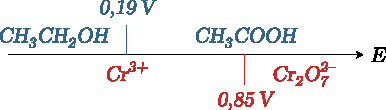
\includegraphics[scale=1]{predom_ch3cooh}
		\end{center}
		On voit bien que la réaction prépondérante est favorisée puisque les domaines
		de prédominance des réactifs sont disjoints~! Par ailleurs, comme la
		différence de $E^\circ$ est grande (i.e., $> \SI{0.20}{V}$), elle sera en
		effet totale.
	}%
\QR{%
	Déterminer la quantité de matière d'alcool expirée par litre d'air, dans
	l'hypothèse d'une alcoolémie atteignant le seuil de \SI{0.50}{g.L^{-1}}
	d'alcool dans un litre de sang.
}{%
	À la limite tolérée dans le sang, on a la concentration massique
	\begin{gather*}
		c_{m,\rm sang} = \SI{0.50}{g.L^{-1}}
		\qor
		c_{m,\rm air} = \frac{c_{m,\rm sang}}{\num{2100}}
		\qet
		c\ind{air} = \frac{c_{m, \rm air}}{M\ind{éthanol}}
		\Lra
		c\ind{air} = \frac{c_{m,\rm sang}}{\num{2100}M\ind{éthanol}}
		\\\AN
		\xul{c\ind{air} = \SI{5.2e-6}{mol.L^{-1}}}
	\end{gather*}
}%
\QR{%
	En déduire la masse de dichromate de potassium devant être placée avant le
	trait de jauge afin que celui-ci indique le seuil limite.
}{%
	Il faut comprendre comment le système fonctionne, et pour ça rien de mieux
	qu'un schéma. On a un ballon de volume $V = \SI{1}{L}$ rempli d'air \textit{a
		priori} à la concentration $c\ind{air}$ en éthanol, soit une quantité $n_a =
		c\ind{air}V = \SI{5.2e-6}{mol}$.
	\smallbreak
	Au-dessus de ce ballon se situe l'éthylotest, dans lequel se trouvent des
	cristaux de dichromate de potassium qui se colorient en vert (présence d'ions
	$\ce{Cr^3+}$) au contact de l'alcool de l'air. Ainsi, on suppose que le trait
	de jauge mentionné dans l'exercice doit faire référence à une limite placée
	sur l'appareil pour que l'utilisateur-ice puisse repérer le seuil toléré pour
	la conduite.
	\smallbreak
	Si on veut que cette limite corresponde à la quantité $n_a$ d'alcool dans
	l'air, c'est donc que la quantité de matière de dichromate qui réagit jusqu'à
	ce trait de jauge est introduit en \textbf{proportions stœchiométriques} avec
	l'éthanol de l'air. C'est en fait une sorte de dosage par titrage, et on
	cherche la relation à l'équivalence~!
	\smallbreak
	En dressant un rapide tableau d'avancement, on trouve la relation
	\begin{gather*}
		n\ind{dichromate} = n_i - 2 \xi_f = 0
		\qet
		n\ind{éthanol} = n_a - 3 \xi_f = 0
		\qso
		\xi_f = \frac{n_i}{2} = \frac{n_a}{3}
		\Lra
		n_i = \frac{2}{3}n_a
		\\
		\beforetext{Pour la masse}
		\boxed{m_i = \frac{2}{3}n_a\,M_{\ce{K_2CR_2O_7}}}
		\Ra
		\xul{m_i = \SI{1.0}{mg}}
	\end{gather*}
}%

\resetQ
\section{Pile argent-zinc}
\enonce{%
On s'intéresse à une pile schématisée par
$\ce{Ag_{\rm(s)}|{Ag}^+_{\rm(aq)}||{Zn}^2+_{\rm(aq)}|Zn_{\rm(s)}}$, avec
$[\ce{Ag+}]_i = c = \SI{0.18}{mol.L^{-1}}$ et $[\ce{Zn^2+}]_i = c' =
	\SI{0.30}{mol.L^{-1}}$. Le compartiment de gauche a un volume $V =
	\SI{100}{mL}$, celui de droite un volume $V' = \SI{250}{mL}$.
\begin{tcb}(data)<lfnt>{Données}
	$E^\circ(\ce{Zn^2+/Zn}) = \SI{-0.76}{V}$ et $E^\circ(\ce{Ag^+/Ag}) =
		\SI{0.80}{V}$.
\end{tcb}
}%
\QR{%
	Déterminer la f.é.m.\ de la pile. Identifier alors l'anode et la cathode par
	un raisonnement sur le trajet des électrons.
}{%
	La f.é.m.\ de la pile est la différence entre les \textbf{potentiels rédox}
	des deux électrodes \textbf{dans la situation initiale} avant qu'elle n'ait
	commencé à débité, donnés par la relation de \textsc{Nernst}. On écrit donc
	les demi-équations et les potentiels associés avant de faire la différence~:
	\begin{gather*}
		\ce{Ag_{\rm(s)} = {Ag}^+_{\rm(aq)} + e^-}
		\quad \Ra \quad
		E_{\ce{Ag^{+}/Ag}} = E^\circ_{\ce{Ag/Ag^+}} + \num{0.06} \log c = \SI{0.76}{V}
		\\
		\ce{Zn_{\rm(s)} = {Zn}^2+_{\rm(aq)} + 2e^-}
		\quad \Ra \quad
		E_{\ce{Zn^{2+}/Zn}} = E^\circ_{\ce{Zn^{2+}/Zn}} + \frac{\num{0.06}}{2} \log
		c' = \SI{-0.78}{V}
		\\\Lra
		\boxed{e = \abs{\Delta{E}} = \SI{1.54}{V}}
	\end{gather*}
	puisque la f.é.m.\ est forcément positive.
	\bigbreak
	Dans un circuit, les électrons migrent du \textbf{potentiel le plus bas} vers
	le \textbf{potentiel le plus haut} ($\Ff\ind{lorentz} = q\Ef$ et $\Ef$
	analogue à $\gf$ donc va des potentiels les plus hauts aux potentiels les plus
	bas, mais $q\ind{électron} = -e$ donc $\Ff$ dans le sens opposé), donc ici du
	\textbf{zinc vers l'argent}. Or, par définition, c'est \textbf{l'oxydation qui
		créé les électrons}, et \textbf{la réduction qui les consomme}~; forcément, à
	l'électrode de zinc il y a formation d'électrons et à l'électrode d'argent il
	y a réception~; ce sont donc respectivement \textbf{l'anode} et \textbf{la
		cathode}.
}%
\QR{%
	Écrire les réactions électrochimiques aux électrodes, puis la réaction de
	fonctionnement qui se produit lorsque la pile débite.
}{%
	\leavevmode\vspace*{-15pt}\relax
	\begin{align*}
		\ce{
		{Ag}^+_{\rm(aq)} + e^-           & = Ag_{\rm(s)}
		}
		\tag*{cathode = réduction}
		\\
		\ce{
		Zn_{\rm(s)}                      & = {Zn}^2+_{\rm(aq)} + 2e^-
		}
		\tag*{anode = oxydation}
		\\\Ra
		\beforetext{on compense les électrons}
		\ce{
		2 {Ag}^+_{\rm(aq)} + Zn_{\rm(s)} & =
		2 Ag_{\rm(s)} + {Zn^2+}_{\rm(aq)}
		}
	\end{align*}
}%
\QR{%
	Schématiser le déplacement des porteurs de charge dans chaque partie de la
	pile lorsqu'elle débite du courant.
}{%
	\hfill
	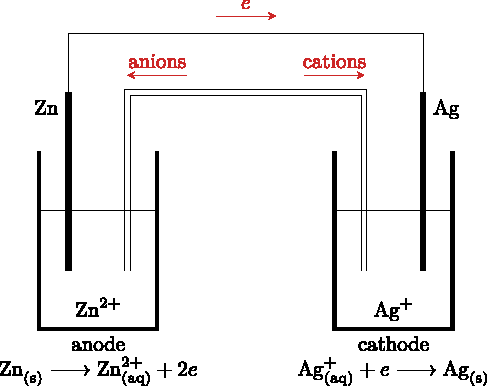
\includegraphics[width=.5\linewidth, valign=t]{pile_ag-zn}
	\hspace*{\fill}
}%
\QR{%
	Déterminer la composition de la pile lorsqu'elle est usée. Quelle quantité
	d'électricité, en coulombs d'abord puis en \si{A.h} ensuite, a-t-elle débité~?
	Ça fait combien de smartphones~?
}{%
	On cherche l'état final. Il nous faut donc la valeur de $K^\circ$. Or, on a
	\[
		K^\circ =
		10^{\DS \frac{2}{\num{0.06}} \abs{\Delta{E^\circ}}} =
		10^{\DS \frac{2}{\num{0.05}} (E^\circ_{\ce{Ag^{+}/Ag}} -
				E^\circ_{\ce{Zn^{2+}/Zn}})}
		\Lra
		\boxed{K^\circ = \num{e53}}
	\]
	On pourra donc \textbf{supposer la réaction totale} (ce qu'on vérifiera après
	coup). On dresse donc le tableau d'avancement, et on fait attention à bien
	faire un \textbf{bilan en quantité de matière} puisque les volumes sont
	différents~:
	\begin{center}
		\def\rhgt{0.35}
		\centering
		\begin{tabularx}{\linewidth}{|l|c||YdYdYdY|}
			\hline
			\multicolumn{2}{|c||}{
				$\xmathstrut{\rhgt}$
			\textbf{Équation}}       &
			$2\ce{{Ag}^+_{\rm(aq)}}$ & $+$       &
			$\ce{Zn_{\rm(s)}}$       & $\ra$     &
			$2\ce{Ag_{\rm(s)}}$      & $+$       &
			$\ce{Zn^{2+}}$                         \\
			\hline
			$\xmathstrut{\rhgt}$
			Initial                  & $\xi = 0$ &
			$cV$                     & \vline    &
			excès                    & \vline    &
			excès                    & \vline    &
			$c'V'$                                 \\
			\hline
			$\xmathstrut{\rhgt}$
			Final                    & $\xi_f$   &
			$cV - 2\xi_{f} = \ep V$  & \vline    &
			excès                    & \vline    &
			excès                    & \vline    &
			$c'V' + \xi_{f}$                       \\
			\hline
		\end{tabularx}
	\end{center}
	En supposant la réaction totale, on a donc $\xi_f = \xi\ind{max} = \frac{cV}{2}$, soit
	\[
		[\ce{Zn^2+}]_f = \frac{c'V' + \frac{cV}{2}}{V'}
		\Lra
		\boxed{
			[\ce{Zn^2+}]_f = c' + \frac{cV}{2V'}
		}
		\Ra
		\xul{
			[\ce{Zn^2+}]_f = \SI{0.34}{mol.L^{-1}}
		}
	\]
	On \textbf{vérifie l'hypothèse de totalité} en appelant $\ep$ la concentration
	de $\ce{Ag^+}$ restante, et on la trouve grâce à la constante de réaction~:
	\[
		K^\circ = \frac{[\ce{Zn^2+}]_fc^\circ}{\ep^2}
		\Lra
		\boxed{\ep = \sqrt{\frac{[\ce{Zn^2+}]_f}{K^\circ}}}
		\Ra
		[\ce{Ag^+}]_f = \SI{1.8e-27}{mol.L^{-1}}
	\]
	Ce qui est bien négligeable~: \textbf{l'hypothèse est validée \iconchek}.
	\bigbreak
	On trouve la quantité d'électricité en multipliant la quantité de matière
	d'électrons échangés ($n_{\ce{e^-},\rm tot}\xi_f$) par la charge électrique
	d'une mole d'électrons ($\Fc = \Nc_A e$)~:
	\[
		Q = 2\xi_f \cdot \Fc
		\Lra
		\boxed{Q = cV \Fc}
		\Ra
		\xul{Q = \SI{1.7e4}{C} = \SI{4.7}{A.h}}
	\]
	Un smartphone gourmand tourne autour des $\SI{4000}{mA.h}$, soit
	$\SI{4}{A.h}$~: ça fait donc suffisamment de charge pour \num{1.2}
	smartphone~!
}%

\resetQ
\section{Stabilisation du cuivre I par précipitation}
\enonce{%
	L'objectif de cet exercice est d'étudier la stabilisation du cuivre de
	$\no{\ce{Cu}} = \myRoman{+1}$ par précipitation, qui illustre plus
	généralement l'influence de la précipitation sur l'oxydoréduction.
	\begin{tcb}(data)<lfnt>{Données}
		$E^\circ(\ce{Cu^+/Cu}) = E_1^\circ = \SI{0.52}{V}$~;
		$E^\circ(\ce{Cu^2+/Cu^+}) = E_2^\circ = \SI{0.16}{V}$
	\end{tcb}
}%
\QR{%
	Montrer à partir de diagrammes de stabilité que l'ion \ce{Cu^+} est instable.
	Pour simplifier, on prendra \SI{1}{mol.L^{-1}} comme concentration frontière.
	Qu'observe-t-on~?
}{%
	\noindent
	\begin{minipage}[t]{.75\linewidth}
		On trace une échelle en potentiels limites, ici confondables avec les
		potentiels standard puisque les concentrations sont unitaires, et on voit que
		la \textbf{réaction prépondérante} est celle de \textbf{la dismutation} et
		qu'\textbf{elle est favorisée} (gamma sens direct)~: $\ce{Cu^+}$ est donc bien
		instable.
		\smallbreak
		On trouve la même chose avec un diagramme de prédominance~:
		\begin{center}
			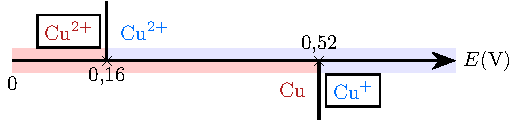
\includegraphics[scale=1]{predom_cu}
		\end{center}
	\end{minipage}
	\hfill
	\begin{minipage}[t]{.25\linewidth}
		\vspace{0pt}
		\begin{center}
			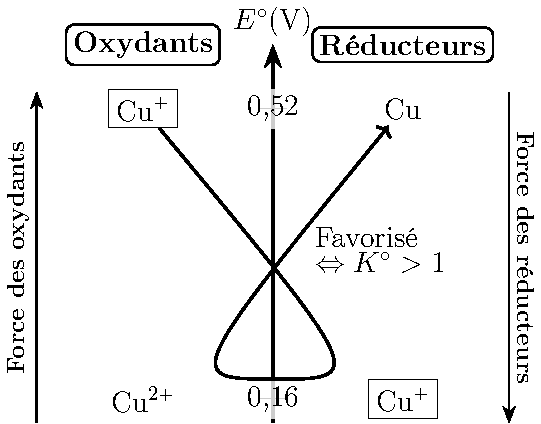
\includegraphics[width=\linewidth]{estand_dismut-cu}
		\end{center}
	\end{minipage}
}%
\enonce{%
	Les ions cuivre I forment avec les ions iodure \ce{I^-} le précipité
	$\ce{CuI_{\rm(s)}}$, de produit de solubilité $K_s = \num{e-11}$.
}%
\QR{%
	Écrire l'équation de dissolution du précipité, puis les demi-équations rédox
	pour les couples \ce{CuI/Cu} et \ce{Cu^2+/CuI}.
}{%
	\leavevmode\vspace*{-15pt}\relax
	\begin{align*}
		\beforetext{Dissolution}
		\ce{
		CuI_{\rm(s)} & = {Cu}^+_{\rm(aq)} + {I}^-_{\rm(aq)}
		}
		\tag*{$K_s$}
		\\
		\beforetext{Couple \ce{CuI/Cu}}
		\ce{
		{Cu}_{\rm(s)} + {I}^-_{\rm(aq)}
		             & =
		CuI_{\rm(s)} + e^-
		}
		\tag*{$E_3$}
		\\\beforetext{Couple \ce{Cu^2+/CuI}}
		\ce{
		CuI_{\rm(s)}
		             & =
		{Cu}^2+_{\rm(aq)} + {I}^-_{\rm(aq)} + e^-
		}
		\tag*{$E_4$}
	\end{align*}
}%
\QR{%
	En déduire la relation de \textsc{Nernst} pour les couples \ce{CuI/Cu} et
	\ce{Cu^2+/CuI} en notant leurs potentiels standard $E_3^\circ$ et $E_4^\circ$,
	respectivement. Exprimer alors $E_3^\circ$ en fonction de $\pk[s]$ et
	$E_1^\circ$ d'une part, puis $E_4^\circ$ en fonction de $\pk[s]$ et
	$E_2^\circ$ d'autre part. Calculer les valeurs numériques.
}{%
	\leavevmode\vspace*{-15pt}\relax
	\begin{gather*}
		\beforetext{On a}
		E_3 = E_3^\circ + \num{0.06} \log \frac{c^\circ}{[\ce{I^-}]}
		\qqet
		E_4 = E_4^\circ + \num{0.06}\log \frac{[\ce{Cu^2+}][\ce{I^-}]}{{c^\circ}^2}
	\end{gather*}
	Comme le précipité est présent (sinon les demi-équations n'existeraient pas),
	on est à l'équilibre du solide en solution saturée, soit
	\begin{gather*}
		K_s = \frac{[\ce{Cu^+}][\ce{I^-}]}{{c^\circ}^2}
		\tag{S}
		\\\Lra
		\frac{[\ce{I^-}]}{c^\circ} = \frac{c^\circ K_s}{[\ce{Cu^+}]}
		\tag{I}
		\\\beforetext{Unicité potentiel $\Ra$}
		E_1 = E_3
		\Lra
		E_1^\circ + \num{0.06} \log \frac{[\ce{Cu^+}]}{c^\circ} =
		E_3^\circ + \num{0.06} \log \frac{c^\circ}{[\ce{I^-}]}
		\\\Lra
		E_3^\circ = E_1^\circ + \num{0.06} \log \frac{[\ce{Cu^+}][\ce{I^-}]}{{c^\circ}^2}
		\tag*{avec (S)}
		\\\Lra
		\boxed{E_3^\circ = E_1^\circ - \num{0.06}\pk[s]}
		\Ra
		\xul{E_3^\circ = -\SI{0.14}{V}}
		\\
		\beforetext{Également,}
		E_2 = E_4
		\Lra
		E_2^\circ + \num{0.06} \log \frac{[\ce{Cu^2+}]}{[\ce{Cu^+}]} =
		E_4^\circ + \num{0.06} \log \frac{[\ce{Cu^2+}][\ce{I^-}]}{{c^\circ}^2}
		\\\Lra
		E_2^\circ + \num{0.06} \log \frac{[\ce{Cu^2+}]}{[\ce{Cu^+}]} =
		E_4^\circ + \num{0.06} \log \frac{[\ce{Cu^2+}]K_s}{[\ce{Cu^+}]}
		\tag*{avec (I)}
		\\\Lra
		\boxed{E_4^\circ = E_2^\circ + \num{0.06}\pk[s]}
		\Ra
		\xul{E_4^\circ = \SI{0.82}{V}}
	\end{gather*}
}%
\QR{%
	Expliquer alors en quoi les ions cuivre I sont stabilisés en présence d'ions
	iodure.
}{%
	\noindent
	\begin{minipage}[t]{.70\linewidth}
		La question n'est pas de discuter de la stabilité des ions
		$\ce{{Cu}^+_{\rm(aq)}}$, mais du \textbf{cuivre au \no +\myRoman{1}}. Sous la
		forme ionique, en effet il y a spontanément dismutation et ils ne sont pas
		stables. En revanche, en présence d'ions iodure ils vont précipiter pour
		former du $\ce{CuI_{\rm(s)}}$, mais le cuivre \textbf{reste au \no
			+\myRoman{1}}. Or, avec une échelle en $E^\circ$, on voit que cette fois la
		réaction de $\ce{CuI_{\rm(s)}}$ sur lui-même est défavorisé~:
		\textbf{$\ce{CuI_{\rm(s)}}$ est stable}, et ainsi le \textbf{cuivre I a été
			stabilité par précipitation}.
	\end{minipage}
	\hfill
	\begin{minipage}[t]{.29\linewidth}
		\vspace{0pt}
		\begin{center}
			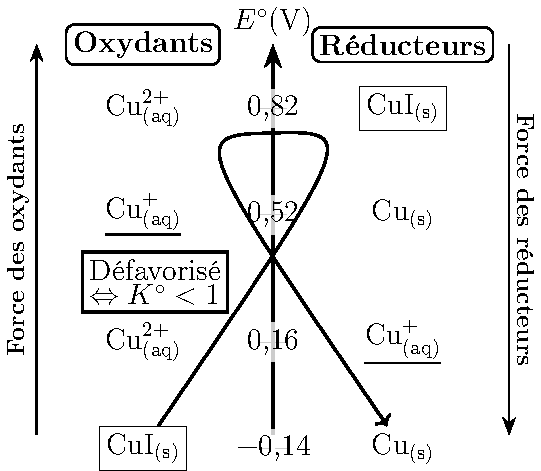
\includegraphics[width=\linewidth]{estand_dismut-cui}
		\end{center}
	\end{minipage}
}%

\resetQ
\section{Dosage colorimétrique en retour}
\enonce{%
	On s'intéresse à un dosage colorimétrique d'une solution de dichromate de
	potassium par les ions fer II en présence d'acide sulfurique, garantissant un
	pH très acide. On donne les potentiels standard
	\[
		E^\circ (\ce{Cr_2O_7^2-/Cr^3+}) = E_1^\circ = \SI{1.33}{V}
		\qet
		E^\circ(\ce{Fe^3+/Fe^2+}) = E_2^\circ = \SI{0.77}{V}
	\]
	En milieu acide, l'ion dichromate est orange et l'ion chrome III est vert,
	alors que l'ion \ce{Fe^2+} est vert pâle et l'ion \ce{Fe^3+} est jaune-orangé.
}%
\QR{%
	Écrire l'équation bilan du titrage rédox direct.
}{%
	\leavevmode\vspace*{-15pt}\relax
	\begin{gather*}
		\beforetext{On a}
		\ce{2 {Cr}^3+_{\rm(aq)} + 7H_2O_{\rm(l)} = {Cr_2O_7}^{2-}_{\rm(aq)} + 14
			{H}^+_{\rm(aq)} + 6 e^-}
		\qet
		\ce{{Fe}^2+ = {Fe}^3+ + e^-}
		\\\Lra
		\boxed{
		\ce{
		{Cr_2O_7}^{2-}_{\rm(aq)} + 14 {H}^+_{\rm(aq)} + 6 {Fe}^2+_{\rm(aq)}
		=
		2 {Cr}^3+_{\rm(aq)} + 7H_2O_{\rm(l)} + 6 {Fe}^3+_{\rm(aq)}
		}
		}
		\tag{1}
		\label{eq:titdir}
	\end{gather*}
}%
\QR{%
	Déterminer l'expression de sa constante d'équilibre, puis la calculer. Cette
	réaction est-elle adaptée à un titrage~? Pourquoi est-elle malgré tout peu
	adaptée à un titrage colorimétrique~?
}{%
	Par unicité du potentiel, on trouve
	\begin{gather*}
		E_1^\circ + \frac{\num{0.06}}{6} \log
		\frac{[\ce{Cr_2O_7^{2-}}][\ce{H^+}]^{14}}{[\ce{Cr^3+}]^2 {c^\circ}^{13}}
		=
		E_2^\circ + \frac{\num{0.06}}{6} \log \frac{[\ce{Fe^3+}]^6}{[\ce{Fe^2+}]^6}
		\\\Lra
		\frac{6}{\num{0.06}} (E_1^\circ - E_2^\circ) =
		\log \frac{[\ce{Fe^3+}]^6}{[\ce{Fe^2+}]^6} - \log \frac{[\ce{Cr_2O_7^{2-}}][\ce{H^+}]^{14}}{[\ce{Cr^3+}]^2 {c^\circ}^{14}}
		\\\Lra
		\frac{6}{\num{0.06}} (E_1^\circ - E_2^\circ) =
		\log \frac{[\ce{Fe^3+}]^6[\ce{Cr^3+}]^2{c^\circ}^{13}}{[\ce{Fe^2+}]^6[\ce{Cr_2O_7^{2-}}][\ce{H^+}]^{14}} =
		\log K^\circ
		\\\Lra
		\boxed{K^\circ = 10^{\DS \frac{6}{\num{0.06}}(E_1^\circ - E_2^\circ)}}
		\Ra
		\xul{K^\circ = \num{e56} \gg 1}
	\end{gather*}
	Cette réaction est donc \textbf{quantitative}, ce qui la rend bien adaptée à
	un titrage (à condition qu'elle soit également rapide). Cependant, elle
	consomme une espèce orange et une espèce verte, et forme une espèce orange et
	une espèce verte~: le \textbf{changement de couleur} à l'équivalence
	\textbf{risque d'être peu visible}.
}%
\QR{%
	Justifier qu'il serait possible de suivre la réaction par potentiométrie.
	Déterminer le sens du saut de potentiel qui serait observé~: est-il descendant
	ou montant~?
}{%
	Cette réaction est une \textbf{réaction rédox}~: on peut donc mesurer son
	potentiel pour rendre compte de sa composition, et ainsi de suivre le titrage.
	\smallbreak
	Pour déterminer le sens du saut de potentiel, il faut déterminer les espèces
	prédominantes de chaque couple avant et après l'équivalence. L'énoncé indique
	(implicitement) que ce sont les ions fer II qui sont ajoutés progressivement
	au milieu. Ainsi~:
	\begin{itemize}
		\bitem{Avant l'équivalence}, $\ce{{Fe}^2+_{\rm(aq)}}$ est limitant, et
		$\ce{{Cr_2O_7^{2-}}_{\rm(aq)}}$ est en excès. Comme la réaction est peu
		avancée au début du titrage, on a peu de $\ce{{Cr}^3+_{\rm(aq)}}$ et de
		$\ce{{Fe}^3+_{\rm(aq)}}$~; ainsi qualitativement
		\[
			\boxed{
			[\ce{Cr_2O_7^{2-}}] > [\ce{Cr^3+}]
			\qet
			[\ce{Fe^3+}] > [\ce{Fe^2+}]
			}
		\]
		c'est-à-dire que ce sont les \textbf{oxydants qui prédominent}, ainsi
		\textbf{le potentiel de la solution est élevé}.
		\bitem{Après l'équivalence}, et vers la fin du titrage,
		$\ce{{Cr_2O_7^{2-}}_{\rm(aq)}}$ est limitant et $\ce{{Fe}^2+_{\rm(aq)}}$ est
		en excès. La réaction n'avance plus et les produits sont présents avec la même
		quantité qu'à l'équivalence, soit
		\[
			\boxed{
			[\ce{Cr_2O_7^{2-}}] < [\ce{Cr^3+}]
			\qet
			[\ce{Fe^3+}] < [\ce{Fe^2+}]
			}
		\]
		donc ce sont les \textbf{réducteurs qui dominent}, et \textbf{le potentiel de
			la solution est faible}.
	\end{itemize}
	En conclusion, le \textbf{saut de potentiel observé est descendant}.
}%
\enonce{%
	Pour contourner la difficulté sans montage de potentiométrie, on effectue un
	dosage en retour. Dans un bécher, on verse $V_1 = \SI{4.0}{mL}$ de la solution
	de dichromate de potassium dont on cherche la concentration $c_1$. On y ajoute
	$V_2 = \SI{10.0}{mL}$ d'une solution de sulfate de fer II en milieu
	sulfurique, de concentration $c_2 = \SI{0.10}{mol.L^{-1}}$ et $V\ind{eau} =
		\SI{90.0}{mL}$ d'eau. On verse ensuite par une burette une solution de
	permanganate de potassium de concentration $c_3 = \SI{1.0e-2}{mol.L^{-1}}$.
	Une coloration violette, caractéristique du permanganate en solution, apparaît
	lorsque que $V_{3,\eqi} = \SI{12}{mL}$ ont été versés.
}%
\QR{%
	Comment peut-on s'assurer qualitativement que les ions fer II ont bien été
	apportés en excès par rapport au dichromate~?
}{%
	On imagine, même si c'est peu explicite, qu'avec un grand excès d'ions fer II
	en solution on aura une couleur verte au lieu de la couleur orangée des ions
	dichromate.
}%
\QR{%
Écrire l'équation bilan du titrage en retour.
}{%
Dans un titrage en retour, on \textbf{dose l'excès connu de réactif}. On peut
cependant s'interroger sur les réactions possibles~: après la première
réaction~\eqref{eq:titdir}, on a les quantités
\[
	\stackunder{$\ce{{Cr_2O_7}^{2-}_{\rm(aq)}}$}{$0$} +
	\stackunder{$\ce{14 {H}^+_{\rm(aq)}}$}{excès} +
	\stackunder{$\ce{6 {Fe}^2+_{\rm(aq)}}$}{$c_2V_2 - 6n_{\ce{Cr_2O_7^{2-}}}$}
	=
	\stackunder{$\ce{2 {Cr}^3+_{\rm(aq)}}$}{$2n_{\ce{Cr_2O_7^{2-}}}$} +
	\stackunder{$\ce{7H_2O_{\rm(l)}}$}{excès} +
	\stackunder{$\ce{6 {Fe}^3+_{\rm(aq)}}$}{$6n_{\ce{Cr_2O_7^{2-}}}$}
\]
donc il serait possible d'utiliser les ions permanganate, très oxydants, pour
réagir avec le réducteur $\ce{Fe^2+}$ ou le réducteur $\ce{Cr^3+}$~; cependant
avec une échelle en $E^\circ$ comme $E^\circ(\ce{Fe^{3+}/Fe^{2+}}) <
	E^\circ(\ce{Cr_2O_7^{2-}/Cr^{3+}})$, c'est bien la réaction avec les ions fer et
le permanganate qui est la réaction prépondérante.
\smallbreak
Ainsi, on écrit les demi-équations~:
\begin{gather*}
	\ce{
	{Fe}^2+_{\rm(aq)} =
		{Fe}^3+_{\rm(aq)} + e^-
	}
	\qet
	\ce{
	{Mn}^2+_{\rm(aq)} + 4 H_2O_{\rm(l)} =
		{MnO_4}^-_{\rm(aq)} + 8 {H}^+_{\rm(aq)} + 5e^-
	}
	\\\Ra
	\boxed{
	\ce{
	{MnO_4}^-_{\rm(aq)} + 8 {H}^+_{\rm(aq)} + 5{Fe}^2+_{\rm(aq)} =
		{Mn}^2+_{\rm(aq)} + 4 H_2O_{\rm(l)} + 5{Fe}^3+_{\rm(aq)}
	}
	}
\end{gather*}
}%
\QR{%
	Déterminer la concentration $c_1$ de la solution de dichromate de potassium.
}{%
	La quantité de dichromate est $c_1V_1$. Le second titrage étant également
	total, à l'équivalence du dosage en retour on aura consommé tout les ions fer
	II restant de la première avec l'ajout d'ions permanganate de la burette, soit
	\begin{gather*}
		c_3V_{3,\eqi} - \xi_f = 0
		\qet
		c_2v_2 - 6c_1V_1 - 5\xi_f = 0
		\\\Lra
		c_3V_{3,\eqi} = \frac{c_2V_2 - 6c_1V_1}{5}
		\Lra
		6c_1V_1 = c_2V_2 - 5 c_3V_{3,\eqi}
		\\\Lra
		\boxed{c_1 = \frac{c_2V_2 - 5c_3V_{3,\eqi}}{6V_1}}
		\Ra
		\xul{c_1 = \SI{1.7e-2}{mol.L^{-1}}}
	\end{gather*}
}%

\resetQ
\section{Pile à combustible à oxyde solide \hfill \small écrit PT 2015}
\enonce{%
Le principe de la pile à combustible consiste à utiliser du dihydrogène pour
stocker et transporter de l'énergie. Une pile à combustible est un assemblage
de cellules élémentaires, en nombre suffisant pour assurer la production
électrochimique d'électricité dans les conditions de tension et d'intensité
voulues. De façon générale, le fonctionnement électrochimique d'une cellule
élémentaire de pile à combustible peut être représenté selon le schéma de la
Figure~\ref{fig:pile_comb}
\begin{center}
	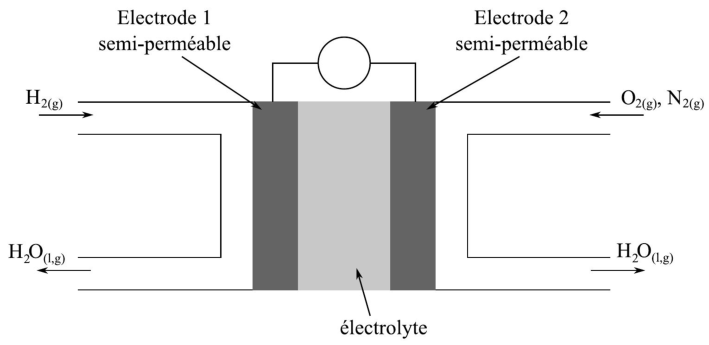
\includegraphics[width=.8\linewidth]{pile_comb}
	\captionof{figure}{Schéma de principe d'une pile à combustible.}
	\label{fig:pile_comb}
\end{center}
Chaque cellule élémentaire est constituée de deux compartiments disjoints,
alimentés chacun en gaz dihydrogène et dioxygène. Les électrodes sont séparées
par un électrolyte solide qui laisse passer les anions oxygène. Les couples
d'oxydoréduction mis en jeu dans la réaction sont
$\ce{{H}^+_{\rm(aq)}/{H_2}_{\rm(g)}}$ et $\ce{{O_2}_{\rm(g)}/H_2O_{\rm(l)}}$.
}%
\QR{%
	Indiquer la position des atomes constitutifs des réactifs et du produit dans
	le tableau périodique. En déduire leur nombre d'électrons de valence et
	ainsi les schémas de \textsc{Lewis} des trois molécules.
}{%
	L'hydrogène est dans la première ligne, première colonne donc 1 électron de
	valence et respecte la règle du duet~; l'oxygène deuxième
	ligne, 16\ieme{} colonne donc 6 électrons de valence et respecte la règle de
	l'octet. Ainsi,
	\[
		\cfig{H-H}
		\qet
		\cfig{\charge{120=\|,-120=\|}{O}=\charge{60=\|,-60=\|}{O}}
		\qet
		\cfig{\charge{45=\|,135=\|}{O}
			(-[7,.7]H)
			(-[5,.7]H)
		}
	\]
}%
\QR{%
	À partir des informations du schéma, attribuer et justifier le choix de la
	cathode et de l'anode aux électrodes 1 et 2, ainsi que le sens de circulation
	des électrons.
}{%
	Au niveau de l'électrode 1, il y a arrivée de dihydrogène, un réducteur, et
	départ d'eau, l'oxydant associé~: il y a donc \textbf{oxydation du
		dihydrogène}, et \textbf{l'électrode 1 est l'anode}. Réciproquement à
	l'électrode 2 il y a arrivée de dioxygène, un oxydant, et départ d'eau qui est
	le réducteur associé~: il y a donc \textbf{réduction du dioxygène}, et
	\textbf{l'électrode 2 est la cathode}. Ainsi, les électrons traversent la pile
	de l'électrode 1 vers l'électrode 2.
}%
\QR{%
Écrire les demi-équations électroniques pour chaque couple mis en jeu, quand
la pile débite.
}{%
D'après la question précédente,
\[
	\ce{{H_2}_{\rm(g)} -> 2 {H}^+_{\rm(aq)} + 2e^-}
	\qet
	\ce{{O_2}_{\rm(g)} + 4 {H}^+_{\rm(aq)} + 4e^- -> 2 {H_2O}_{\rm(l)}}
\]
\begin{tcb}(rema)<lftt>{Signe des demi-équations}
	Il n'est jamais faux d'écrire les demi-équations avec des signes «~=~», mais
	comme la pile débite on suppose qu'on s'intéresse au sens de
	fonctionnement~; on peut insister sur la transformation avec une flèche.
\end{tcb}
}%
\QR{%
	Le réactif qui est oxydé est appelé le combustible de la pile. Parmi les
	espèces chimiques présentes dans les couples, laquelle constitue le
	combustible~?
}{%
	Parmi les espèces en présence, c'est \textbf{le dihydrogène} qui est oxydé,
	c'est donc lui le combustible.
}%
\QR{%
En déduire l'équation de la réaction modélisant la transformation ayant lieu
dans la cellule de réaction.
}{%
En combinant les demi-équations~:
\[
	\boxed{
	\ce{
	2 {H_2}_{\rm(g)} + {O_2}_{\rm(g)} -> 2 {H_2O}_{\rm(l)}
	}
	}
\]
}%
\enonce{%
	Dans un véhicule motorisé fonctionnant grâce à une pile à combustible, on
	estime à \SI{1.5}{kg} la masse de dihydrogène nécessaire pour parcourir
	\SI{250}{km}.
}%

\QR{%
	Calculer la quantité de matière de dihydrogène correspondant à cette masse,
	puis le volume occupé par cette quantité de gaz à $\SI{20}{\degreeCelsius}$
	sous pression atmosphérique.
}{%
	La masse molaire du dihydrogène est $M_{\ce{H_2}} = \SI{2.0}{g.mol^{-1}}$~; la
	quantité de matière nécessaire pour parcourir \SI{250}{km} est donc
	\begin{gather*}
		n = \frac{m}{M} = \SI{750}{mol}
		\\\beforetext{Or, gaz parfait donc}
		\boxed{V = \frac{nRT}{P}}
		\Lra
		\xul{V = \SI{1.8e4}{L}}
	\end{gather*}
}%
\QR{%
	Quel est l'avantage pour l'environnement de l'utilisation d'une pile à
	combustible au dihydrogène par rapport à un carburant classique~? Quel en est
	l'inconvénient majeur~?
}{%
	Le gros avantage de la pile à combustible est qu'elle ne rejette que de l'eau,
	et aucune substance polluante. L'inconvénient majeur de la pile envisagée ici
	est bien sûr la production et le stockage du dihydrogène, qui est un gaz très
	explosif.
	\begin{tcb}(rema)<lftt>{Remarque}
		Le stockage du dihydrogène pour les piles à combustible est un domaine de
		recherche très actif. Il est a priori produit par électrolyse de l'eau
		(i.e.\ l'inverse de la réaction ayant lieu dans la pile), l'énergie
		nécessaire à l'électrolyse pouvant venir d'une source d'énergie propre. Il
		est ensuite stocké selon différentes modalités~: bouteille de gaz ou de
		liquide, stockage dans des hydrures métalliques solides, etc. Voir la page
		Wikipédia «~Pile à combustible~» pour plus d'informations.
	\end{tcb}
}%

\resetQ
\section{Accumulateur lithium métal \hfill \small oral banque PT}
\enonce{%
	On étudie ici l'accumulateur lithium-oxyde de manganèse, qui représente
	environ 80\% du marché des batteries au lithium. La première électrode est en
	dioxyde de manganèse \ce{MnO2}, la deuxième en lithium \ce{Li}. Ces deux
	électrodes baignent dans un électrolyte organique contenant des ions \ce{Li+}.
	\begin{tcb}(data)<lfnt>{Données}
		\begin{itemize}
			\item Numéro atomique du lithium~: $Z = 3$.
			\item Masse molaire du lithium~: $M_{\ce{Li}} = \SI{5.9}{g.mol^{-1}}$.
			\item Potentiels standard~: $E_1^\circ(\ce{Li^+/Li_{\rm(s)}}) =
				      -\SI{3.03}{V}$ et
			      $E_2^\circ(\ce{{MnO_2}_{\rm(s)}/{LiMnO_2}_{\rm(s)}})$ = \SI{0.65}{V}.
		\end{itemize}
	\end{tcb}
}%
\QR{%
	Indiquer la position du lithium dans le tableau périodique. Pourquoi choisir
	un électrolyte organique plutôt que de l'eau~?
}{%
	Le lithium est situé deuxième ligne, première colonne, sous l'hydrogène. C'est
	le premier métal alcalin. Comme tous les alcalins, c'est un \textbf{très fort
		réducteur}, qui réagit violemment avec l'eau (de manière explosive).
}%
\QR{%
	Écrire les réactions aux électrodes lorsque l'accumulateur fonctionne en
	générateur, ainsi que la réaction globale de fonctionnement.
}{%
	\noindent
	\begin{minipage}[t]{.55\linewidth}
		En fonctionnement générateur, la réaction chimique a lieu dans le sens
		spontané, donc entre espèces de domaines disjoints. On trace le diagramme de
		prédominance~:
	\end{minipage}
	\hfill
	\begin{minipage}[t]{.45\linewidth}
		\begin{center}
			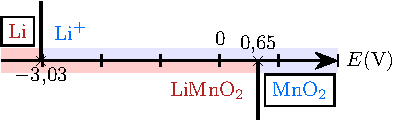
\includegraphics[width=.7\linewidth]{predom_limno}
		\end{center}
	\end{minipage}
	\smallbreak
	D'où les demi-équations~:
	\begin{align*}
		\beforetext{Électrode de lithium}
		\ce{Li_{\rm(s)}                                   & -> {Li}^+_{\rm(aq)} + e^-}
		\\\beforetext{Électrode de manganèse}
		\ce{{MnO_2}_{\rm(s)} + {Li}^+_{\rm(aq)} + e^-     & -> {LiMnO_2}_{\rm(s)}}
		\\\beforetext{Fonctionnement global}
		\ce{
		{MnO_2}_{\rm(s)} + {Li}^+_{\rm(aq)} + Li_{\rm(s)} & ->
		{LiMnO_2}_{\rm(s)} + {Li}^+
		}
		\\\beforetext{Soit}
		\ce{
		{MnO_2}_{\rm(s)} + Li_{\rm(s)}                    & ->
		{LiMnO_2}_{\rm(s)}
		}
	\end{align*}
	\begin{tcb}(rema)<lftt>{Remarque}
		L'ion lithium joue un rôle analogue à celui des ions $\ce{H^+}$ en solution
		aqueuse.
	\end{tcb}
}%
\QR{%
	La pile contient-elle un pont salin ou équivalent~? Pourquoi~?
}{%
	Les deux espèces qui réagissent sont deux solides, physiquement séparés en
	deux électrodes. Le rôle du pont salin étant d'empêcher les réactifs d'être en
	contact direct pour force le transfert d'électrons par l'extérieur du système
	(et donc être exploitables), il n'y a pas de pont salin nécessaire ici.
}%
\QR{%
	Déterminer la force électromotrice de la pile.
}{%
	\leavevmode\vspace*{-15pt}\relax
	\begin{gather*}
		E_{\ce{Li}} = E_1^\circ + \num{0.06}\log \frac{[\ce{Li^+}]}{c^\circ}
		\qet
		E_{\ce{MnO_2}} = E_2^\circ + \num{0.06} \log \frac{[\ce{Li^+}]}{c^\circ}
		\\\Ra
		e = E_{\ce{MnO_2}} - E_{\ce{Li}}
		\Lra
		\boxed{e = E_2^\circ - E_1^\circ}
		\Ra
		\xul{e = \SI{3.68}{V}}
	\end{gather*}
}%
\QR{%
	Déterminer la capacité $C$ de la pile en \si{A.h} pour une masse initiale de
	\SI{2}{g} de lithium.
}{%
	À partir de l'équation à l'électrode de lithium, on constate que lorsque la
	réaction (totale) est terminée, la quantité de matière $n$ d'électrons ayant
	transité dans le circuit est égale à la quantité de matière de lithium
	initialement introduite. D'où la charge totale~:
	\[
		\boxed{C = \frac{m_{\ce{Li}}}{M_{\ce{Li}}} \Nc_A e}
		\Ra
		\xul{C = \SI{3.2e4}{C} = \SI{9.0}{A.h}}
	\]
}%

\resetQ
\section{Dosage d'une solution d'hypochlorite de sodium \hfill \small écrit PT
  2016}

\enonce{%
Après avoir introduit un volume $V_0 = \SI{2.00}{mL}$ d'une solution
commerciale d'hypochlorite de sodium $(\ce{Na^+}~;~\ce{ClO^-})$ dans une fiole
jaugée de volume $V_f = \SI{100}{mL}$, on complète avec de l'eau distillée
jusqu'au trait de jauge. À un volume $V = \SI{10.0}{mL}$ de cette solution
fille, on ajoute environ \SI{10}{mL} d'une solution d'iodure de potassium
$(\ce{K^+}~;~\ce{I^-})$ à 15\% en masse et \SI{5.0}{mL} d'acide éthanoïque
$\ce{CH_3CO_2H_{\rm(aq)}}$ à \SI{3.0}{mol.L^{-1}}. L'échantillon obtenu est
titré par une solution de thiosulfate de sodium
$(\ce{2Na^+}~;~\ce{{S_2O_3}^{2-}})$ de concentration $c =
	\SI{2.0e-2}{mol.L^{-1}}$. Le volume équivalent est égal à $V' =
	\SI{16.0}{mL}$.
\begin{tcb}(data)<lftt>{Données à \SI{298}{K}}
	\[
		E^\circ(\ce{ClO^-/Cl^-}) = \SI{0.89}{V}
		\qquad
		E^\circ(\ce{I_{2}/I^-}) = \SI{0.54}{V}
		\qquad
		E^\circ(\ce{{S_4O_6}^2-/{S_2O_3}^2-}) = \SI{0.08}{V}
	\]
\end{tcb}
}%
\QR{%
	Proposer une équation pour la réaction entre les ions hypochlorite
	$\ce{ClO^-}$ et les ions iodure \ce{I^-}. Prévoir qualitativement le caractère
	favorisé ou défavorisé de la réaction.
}{%
	\leavevmode\vspace*{-15pt}\relax
	\begin{align*}
		\beforetext{Couple $\ce{ClO^-/Cl^-}$}
		\ce{{Cl}^-_{\rm(aq)} + H_2O_{\rm(l)}          & = {ClO}^- + 2 {H}^+_{\rm(aq)} + 2e^-}
		\tag{1}
		\\
		\beforetext{Couple $\ce{I_{2}/I^-}$}
		\ce{2 {I}^-_{\rm(aq)}                         & = {I_2}_{\rm(aq)} + 2e^-}
		\tag{2}
		\\\beforetext{Réaction}
		\ce{
		{ClO}^- + 2 {H}^+_{\rm(aq)} 2 {I}^-_{\rm(aq)} & =
		{Cl}^-_{\rm(aq)} + {I_2}_{\rm(aq)} + H_2O_{\rm(l)}
		}
		\tag*{$(3) = (2) - (1)$}
	\end{align*}
	On trace un diagramme de prédominance qualitatif (avec le potentiel frontière
	égal au potentiel standard) pour montrer que les deux espèces ont des domaines
	disjoints, et donc que la réaction est favorisée~:
	\begin{center}
		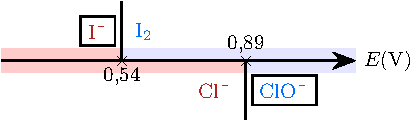
\includegraphics[width=.5\linewidth]{predom_cli}
	\end{center}
}%
\QR{%
Proposer une équation pour la réaction de titrage du diiode \ce{I2} par les
ions thiosulfate $\ce{S_2O_3^{2-}}$. Prévoir qualitativement le caractère
favorisé ou défavorisé de la réaction.
}{%
\leavevmode\vspace*{-15pt}\relax
\begin{align*}
	\beforetext{Couple $\ce{S_4O_6^2-/S_2O_3^2-}$}
	\ce{2 {S_2O_3}^{2-}_{\rm(aq)}                 & = {S_4O_6}^{2-}_{\rm(aq)} + 2e^-}
	\tag{1}
	\\
	\beforetext{Couple $\ce{I_{2}/I^-}$}
	\ce{2 {I}^-_{\rm(aq)}                         & = {I_2}_{\rm(aq)} + 2e^-}
	\tag{2}
	\\\beforetext{Réaction}
	\ce{
	{ClO}^- + 2 {H}^+_{\rm(aq)} 2 {I}^-_{\rm(aq)} & =
	{Cl}^-_{\rm(aq)} + {I_2}_{\rm(aq)} + H_2O_{\rm(l)}
	}
	\tag*{$(3) = (1) - (2)$}
\end{align*}
On trace un diagramme de prédominance qualitatif (avec le potentiel frontière
égal au potentiel standard) pour montrer que les deux espèces ont des domaines
disjoints, et donc que la réaction est favorisée~:
\begin{center}
	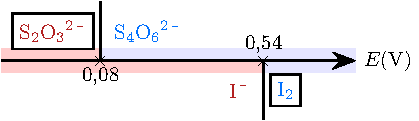
\includegraphics[width=.5\linewidth]{predom_i2s2o3}
\end{center}
}%
\QR{%
Sachant que les ions iodure et l'acide éthanoïque sont introduits en excès,
déterminer la concentration en ions hypochlorite dans la solution commerciale.
}{%
Raisonnons d'abord sur la deuxième réaction pour déterminer la quantité de
matière $n_1$ de diiode formée par la première réaction. À l'équivalence, le
thiosulfate est apporté dans les proportions stœchiométriques par rapport au
diiode, un bilan de matière montre donc que
\[
	n_1 - \xi\ind{eq} = 0
	\qet
	cV' - 2\xi\ind{eq} = 0
	\Lra
	\boxed{n_1 = \frac{cV'}{2}}
\]
Considérons la première réaction totale. Comme le réactif limitant est par
hypothèse l'ion hypochlorite $\ce{{ClO}^-_{\rm(aq)}}$, un bilan de matière
montre que la quantité de matière initiale d'ion hypochlorite est égale à la
quantité de matière de diiode formé, c'est-à-dire $n_1$. Ainsi, compte-tenu du
processus de préparation des solutions,
\[
	n_1 = Vc_f
	\Lra
	c_f = \frac{n_1}{V}
\]
et par conservation de la matière au cours de la dilution, on a la
concentration $c_0$ de la solution commerciale~:
\[
	c_0 V_0 = c_fV_f
\]
D'où en rassemblant,
\[
	c_0 = \frac{V_f}{V_0}c_f = \frac{V_f}{V_0}\frac{n_1}{V}
	\Lra
	\boxed{c_0 = \frac{V_fV'}{2V_0V}C}
	\Ra
	\xul{c_0 = \SI{8.0e-1}{mol.L^{-1}}}
\]
}%

\end{document}
